\newcommand{\figureProtocolClassification}[1]{
  \def\lang{\detokenize{#1}}
  \def\langRu{\detokenize{ru}}
  \def\langEn{\detokenize{en}}
  \def\figureCaption{XXX: No translation.}
  \def\figureDataTransfer{XXX: No translation.}
  \def\figureParallel{XXX: No translation.}
  \def\figureSerial{XXX: No translation.}
  \ifx \lang\langRu
  \def\figureCaption{
    Классификация методов передачи данных.
  }
  \def\figureDataTransfer{Передача данных}
  \def\figureParallel{Параллельная}
  \def\figureSerial{Последовательная}
  \fi
  \ifx \lang\langEn
  \def\figureCaption{
    Classification of data transferring methods.
  }
  \def\figureDataTransfer{Data transfer}
  \def\figureParallel{Parallel}
  \def\figureSerial{Serial}
  \fi
  \begin{figure}[H]
    \centering
    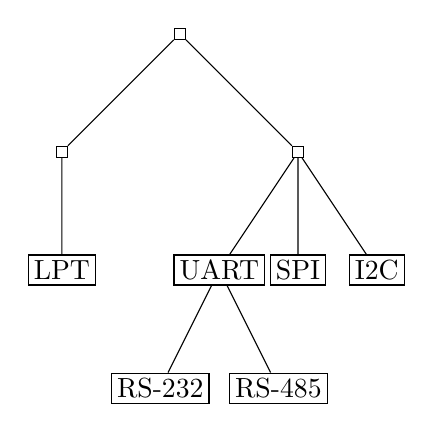
\begin{tikzpicture}[
        level distance=15mm,
        level 1/.style={sibling distance=30mm},
        level 2/.style={sibling distance=10mm},
        level 3/.style={sibling distance=15mm},
        every node/.style={rectangle,draw,inner sep=2pt},
      ]
      \node {\figureDataTransfer}
      child {node {\figureParallel}
        child {node {LPT}}
      }
      child {node {\figureSerial}
        child {node {UART}
          child {node {RS-232}}
          child {node {RS-485}}
        }
        child {node {SPI}}
        child {node {I2C}}
      };
    \end{tikzpicture}
    \caption{\figureCaption}
    \label{fig:communication-data-transfer-categories}
  \end{figure}
}
